
\documentclass[a4paper,12pt]{report}


\usepackage[english,romanian]{babel}
\usepackage{pgfpages}
\usepackage{graphicx}

\usepackage{ucs}
\usepackage[utf8x]{inputenc}
% 
% \newcommand{\texten}[1]{\foreignlanguage{english}{#1}}
% \newcommand{\textro}[1]{\foreignlanguage{romanian}{#1}}
% 
% \newcommand{\sh}[0]{\textcommabelow{s}}		%pentru ş cu virgulă
% \newcommand{\tz}[0]{\textcommabelow{t}}		% pentru ţ cu virgulă

\usepackage[unicode]{hyperref}
\usepackage[T1]{fontenc}
\usepackage{tikz}
% \usepackage{colortbl}
\usepackage{yfonts}

\usepackage{amssymb,amsmath}
\usepackage{amsthm}

\usepackage{paralist}

\usepackage{enumerate}

% \usepackage{makeidx}
% \usepackage{showidx}

\usepackage{multirow}

% \usepackage{float}

% \usepackage{subfig}

% \usepackage{multirow}
% \usepackage{rotating}

% \usepackage[ruled,vlined,longend]{algorithm2e}
% \SetAlFnt{\small}

% \usepackage{program}
\usepackage{algpseudocode}

\usepackage{verbatim}

\usepackage{listings}

\lstset{
	language=C,
%	basicstyle=\ttfamily,
	basicstyle=\small\ttfamily,
	keywordstyle=\bfseries,
	commentstyle=\itshape,
	escapechar=\,
	emphstyle=\bfseries\color{red}
 	commentstyle=\slshape\color{green!50!black},
 	keywordstyle=\bfseries\color{blue!50!black},
 	identifierstyle=\color{blue},
 	stringstyle=\color{orange},
	showstringspaces=false
}

\usepackage{setspace}
% \usepackage{tocbibind}
% \usepackage{fancyhdr}


% \newcommand{\OSName}{\textit{Nachos}}
\newcommand{\OSName}{\textit{HAL9000}}

\title{The Design of \OSName{} Operating System}

\author{Students' Name}

% \onehalfspacing

\begin{document}

\selectlanguage{english}
% \selectlanguage{romanian}


\maketitle

\begin{abstract}
The abstract should contain a very short description of the results presented in this report. 

Take into account that a design document is a high-level, logical (abstract) description of the solution you propose to the problems and requirements you dealt with. Though, it should be detailed enough such that somebody who already knows and understands the requirements could implement (i.e. write the code) the design without having to take any significant additional design decisions. Even further, if such an implementer would happen to be an experienced one, he or she should be able to use the design document to implement the solution in just few hours (not necessarily including the debugging). 

\textbf{Important notes}. Take care to remove from the given design document template all the text that was given to you as a guideline and provide your own document with only your own original text. Also, do not simply write anything in any section just to have some text there, but only write text that makes sense in the given context. We will not count the number of pages or words of your document, but will only evaluate the meaning and completeness of the written words. 
\end{abstract}


\chapter{General Presentation}

\section{Working Team}

Specify the working team members' names and their responsibility.

\begin{enumerate}
	\item Firstname1 Familyname1 
	    \begin{enumerate}
	     \item Threads: dealt with AAA
	     \item Userprog: dealt with BBB
	     \item VM: dealt with CCC
	    \end{enumerate}

	\item Firstname2 Familyname2
	    \begin{enumerate}
	     \item Threads: dealt with AAA
	     \item Userprog: dealt with BBB
	     \item VM: dealt with CCC
	    \end{enumerate}
	    
	\item Firstname3 Familyname3
	    \begin{enumerate}
	     \item Threads: dealt with AAA
	     \item Userprog: dealt with BBB
	     \item VM: dealt with CCC
	    \end{enumerate}

	   
\end{enumerate}


% \section{System}


\chapter{The (One) Way to Proceed for Getting a Reasonable Design}

\section{General Considerations}

There are multiple strategies to develop a software application, though basically all of them comprise the following four phases:
\begin{enumerate}
    \item establish the \textit{application requirements} or specification;
    \item derive the ways the requirements can be realized / satisfied, i.e. \textit{designing} the application;
    \item \textit{implement} the design, e.g. write the corresponding code;
    \item check if the implementation satisfies the specification, at least by \textit{testing} (as exhaustive as possible) the developed application.
\end{enumerate}

In practice, a perfect and complete design is not entirely possible from the beginning for most of the projects. So, at least the last three phases actually correspond to a progressive and repeating process, i.e. make a first design, implement it, test the resulting code, see what is working bad or missing functionality, go back and change the design, make the corresponding code changes or additions, test them again and so on. 

I want, however, to warn you that even if we cannot make a perfect design from the beginning that does not mean that we do not have to make any design at all and just start writing code. This is a really bad idea. And actually, in my opinion, when you start writing code without a more or less formal design, what you actually have to do is to derive an on-the-fly design. What I mean is that you cannot just write ``some'' code there, hoping to get the required functionality. You must think of \textit{how} to code and \textit{what} code to write and this is basically a (hopefully, logical) plan, i.e. a design. Such a strategy, however, results most of the time and for most of the people in just poorly improvisation and requires many returns to the ``design'' phase to change data structures and code. In short, a lot of lost time and bad results. 

Coming back to the idea that we cannot make a complete design from the beginning, there are a few ways to understand this and reasons of having it. Firstly, it is generally difficult to cover all the particular cases, especially for very complex systems and requirements. That means that what you get first is a sort of a general design, establishing the main components of your application and their basic interrelationships. It is not surely that you immediately could start writing code for such a design, but it is very possible to be able to write some prototype, just to see if your ideas and design components could be linked together. On way or another, the next major step is to go deeper for a more detailed design. Secondly, one reason of not getting a complete design from the beginning is just because you want to concentrate on a particular component firstly, and only than to cope with the others. However, this is just a particular case of the first strategy, because it is not possible to deal with one application component without knowing firstly which are the others and how they depend on one another. Thirdly, maybe it is not needed to get a complete detailed design from the beginning, just because the application components are dealt with by different teams or, like in your case, different team members. It is not needed in such a case to deal with the complexity of each application component from the beginning, as each one be will be addressed latter by its allocated team (members), but just try to establish as precise as possible, which are the application components and how they need to interact each other. In your \OSName{} project the application components are most of the time already established, so what remains for you is only to clarify the interactions and interfaces between them. After such a general design, each team (member) can get independently into a more detailed design of his/her allocated application component. 
In conclusion, you need to derive at least a general design before starting writing any code and refine that design later. 

Take into  account, however, that in or project we have distinct deadlines for both design and implementation phases, and that you will be graded for the two relatively independent (thus, design regrading will be done only occasionally). This means that you have to try to derive a very good and as detailed as possible design from the beginning.  


Another practical idea regarding the application development phases is that there is no clear separation between those phases and especially between the design and implementation ones. This means that during what we call the design phase we have to decide on some implementation aspects and, similarly, when we are writing code we still have to take some decisions when more implementation alternatives exists (which could influence some of the application non-functional characteristics, like performance) or some unanticipated problems arise. Even taking into account such realities, in this design document we are mainly interested (and so you have to focus) mainly on the design aspects. But, as I said above, I will not expect you providing a perfect design, which would need no changes during its implementation. However, this does not mean that you are free to come with an unrealistic, incoherent, illogical, hasty, superficial design, which does not deal with all the (clear and obvious) given requirements. 

One important thing to keep in mind when you make your design and write your design document is that another team member has to be able to figure out easily what you meant in your design document and implement your design without being forced to take any additional design decisions during its implementation or asking you for clarifications. It is at least your teacher you have to think of when writing your design document, because s/he has to understand what you meant when s/he will be reading your document. Take care that you will be graded for your design document with approximately the same weight as for your implementation. 

Beside the fact that we do not require you a perfect design, and correspondingly we do not grade with the maximum value only perfect designs (yet, please, take care and see again above what I mean by an imperfect design), your design document must also not be a formal document. At the minimum it should be clear and logical and complies the given structure, but otherwise you are free to write it any way you feel comfortable. For example, if you think it helps someone better understand what you mean or helps you better explain your ideas, you are free to make informal hand-made figures, schemes, diagrams, make a photo of them or scan them and insert them in your document. Also, when you want to describe an algorithm or a functionality, you are free to describe it any way it is simpler for you, like for instance as a pseudo-code, or as a numbered list of steps. However, what I generally consider a bad idea is to describe an algorithm as an unstructured text. On one hand, this is difficult to follow and, on the other hand, text could generally be given different interpretations, though as I already mentioned your design should be clear and give no way for wrong interpretation, otherwise it is a bad design. 

Regarding the fact that design and implementation could not be clearly and completely separated, this is even more complicated in your \OSName{} project that you start from a given code of an already functional system. In other words you start with an already partially designed system, which you cannot ignore. This means, on one hand, that you could be restricted in many ways by the existing design and \OSName{} structure and, on the other hand, that you cannot make your design ignoring the \OSName{}' code. Even if, theoretically, a design could be abstract enough to support different implementations (consequently, containing no particular code), your \OSName{} design has to make direct references to some existing data structures and functions, when they are needed for the functionality of the \OSName{} component your are designing. So, do not let your design be too vague (abstract) in regarding to the functionality directly relying on exiting data structures and functions and let it mention them explicitly. For instance, when you need to keep some information about a thread, you can mention that such information will be stored as additional fields of the ``\textit{THREAD}'' data structure. Or, when you need to keep a list of some elements, you have to use the lists already provided by \OSName{} and show that by declaring and defining your list in the way \OSName{} does, like below:

\begin{lstlisting}
	// this is the way HAL9000 declares a generic list
	LIST_ENTRY myCoolList;

	typedef struct _MY_LIST_ELEM {
		... some fields ...

		// this is needed for linking MY_LIST_ELEM in the 
		// myCoolList list
		LIST_ENTRY ListElem;
	} MY_LIST_ELEM, *PMY_LIST_ELEM;
\end{lstlisting}

The next sections illustrate the design document structure we require and describe what each section should refer to.


\section{Application Requirements. Project Specification}

% Describe briefly what you have been given (have started from) at the beginning of the assignment and the way the existing functionality must be extended.

\subsection{``What you have'' and  ``What you have to do''}

In this section you have to make clear what you are required to do for each particular assignment of the \OSName{} project. In the \OSName{} project, you are already given the assignment requirements, so it is not your job to establish them. You must, however, be sure that you clearly understand them. Having no clear idea about what you have to do, gives you a little chance to really get it working. Please, do not hesitate to ask as many questions about such aspects on the \OSName{} forum (on the moodle page of the course) as you need to make all the requirements clear to you. Take care, however, that you have to do this (long enough) before the design deadline, such that to get an answer in time. We will do our best in answering your questions as fast as possible, though we cannot assure you for a certain (maximum) reaction time. You will not excused at all if you say you had not understood some requirements when you will be presenting your design document.

So, for this small section, take a moment and think of and briefly write about: 
\begin{enumerate}
    \item what you are starting from, i.e. what you are given in terms of \OSName{} existing functionality, and
    \item what you are required to do.
\end{enumerate}


\subsection{``How it would be used''}

Making clear the requirements could be helped by figuring some ways the required functionality would be used once implemented. 
For this you have to describe briefly a few common use-cases, which could later be used as some of the implementation tests. 

You could use for this the tests provided with the \OSName{} code in the ``tests/'' subdirectory. Take at least a short look at each test case to identify common cases.


\section{Derive the Application's Design}

Generally, you have to follow a top-down design approach, starting with a particular requirement and identifying the inputs it generates to your application (i.e. \OSName{} OS). Such that you could establish the ``entry (starting) points'' in your system to start your design from. 

Next, you also have to identify the logical objects (i.e. data structures, local and global variables etc.) implied and affected by the analyzed requirement and the operations needed to be performed on them. Also establish if you need to introduce and use additional information (i.e. fields, variables) in order to make such operations possible. 

Once you established the information you need to keep in order to dealt with the analyzed requirement, you could decide on the way to keep track of and manage that data. 
In other words, this is the way you can \textit{identify the needed data structures} and \textit{operations on them}. There could not necessarily be just one solution. For example, at one moment you could use a linked list or a hash table. In order to decide for one or another, you have to figure out which one helps you more, which one fits better for the most frequent operation and other things like these. Once you decided on the data structures, you have to establish where and how they are
\begin{inparaenum}[(1)]
    \item \textit{initialized}, 
    \item \textit{used}, 
    \item \textit{changed}, and finally 
    \item \textit{removed}.
\end{inparaenum}

This way you could identify the places (e.g. other system components, functions) where you have to add the needed functionality. In terms of \OSName{} code you could identify the functions needed to be used, changed or even added. 

As a result of your requirement analysis you could organize your resulting design like below. 

\subsection{Needed Data Structures and Functions}

Describe the \textit{data structures} and \textit{functions} (only their signature and overall functionality) needed by your design and what they are used for. Describe in few words the purpose of new added data structures, fields and functions. As mentioned before, cannot ignore the fact that \OSName{} is written in C. Thus, describe you data structures in the C syntax referring, when the case, to existing data structures, like in the example given above. If you only need to add new fields in existing data structures, mention only the added fields, not all of them. 

\begin{lstlisting}
    typedef struct _EXISTENT_DATA_STRUCTURE {
        ...
        int NewField;
        char NewField2;
        ...
    } EXISTENT_DATA_STRUCTURE, *PEXISTENT_DATA_STRUCTURE;
    
    typedef struct _NEW_DATA_STRUCTURE {
        ... new fields ...
    } NEW_DATA_STRUCTURE, *PNEW_DATA_STRUCTURE;
    
    STATUS NewFunction(void);
\end{lstlisting}


\subsection{Detailed Functionality}

This should be \textbf{the largest and most important section} of you design document. It must describe \textbf{explicitly}, in words and pseudo-code the way your solution works. DO NOT INCLUDE CODE HERE. This is a design document, not a code description one. As much as possible try to describe the design principles, not implementation details. 

Give examples, if you think they can make your explanation clearer. You are free to use any other techniques (e.g. use-case diagrams, sequence diagrams etc.) that you think can make your explanation clearer. See Figure~\ref{fig:sample-image} below to see the way images are inserted in a Latex file. 

\begin{figure}[h]
	\centering
	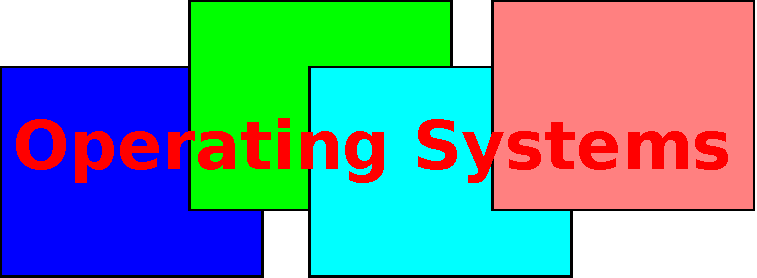
\includegraphics[width=0.5\textwidth]{figures/sample-image.pdf}
	\caption{Sample image}
	\label{fig:sample-image}
\end{figure}

When describing algorithms you are to use or develop, it is very important to also describe them in a formal way, not just as free text description. Commonly, this could be done as a sort of pseudo-code or just as a simple list of logically ordered steps (enumerated list). In your algorithm description you should (i.e. must) refer to the data structures and variables you described in the previous section, following the recommendations in Section~\ref{sec:derive-design}. This way you avoid describing your algorithms too vague and reduce the risks of being misunderstood.  

Here you have a pseudo-code description of an algorithm taken from \\ \href{http://en.wikibooks.org/wiki/LaTeX/Algorithms\_and\_Pseudocode\#Typesetting\_using\_the\_program\_package}{http://en.wikibooks.org/wiki/LaTeX}. It uses the \textit{algpseudocode} package. Alternatively, you can use any other package and environment of same sort you like. 

% \begin{program}
% \mbox{Example of a pseudo-code algorithm description:}
% \BEGIN
%   \FOR i:=1 \TO 10 \STEP 1 \DO
%      |expt|(2,i); \\ |newline|() \OD
% \rcomment{This text will be set flush to the right margin}
% \WHERE
% \PROC |expt|(x,n) \BODY
%           z:=1;
%           \DO \IF n=0 \THEN \EXIT \FI;
%              \DO \IF |odd|(n) \THEN \EXIT \FI;
% \COMMENT{This is a comment statement};
%                 n:=n/2; x:=x*x \OD;
%              \{ n>0 \};
%              n:=n-1; z:=z*x \OD;
%           |print|(z) \ENDPROC
% \END
% \end{program}

\begin{algorithmic}
\If {$i\geq maxval$}
    \State $i\gets 0$
\Else
    \If {$i+k\leq maxval$}
        \State $i\gets i+k$
    \EndIf
\EndIf
\end{algorithmic}

\subsection{Explanation of Your Design Decisions}

Justify very briefly your design decisions, specifying other possible design alternatives, their advantages and disadvantages and mention the reasons of your choice. For instance, you can say that you decided for a simpler and easier to implement alternative, just because you had no enough time to invest in a more complex one. Or just because you felt it would be enough for what \OSName{} tests would check for. This could be viewed as a pragmatical approach and it is not necessarily a bad one, on the contrary, could be very effective in practice.  


\section{Testing Your Implementation}

Please note that the \OSName{} code is provided with a set of tests that are used to check and evaluate your implementation. The \OSName{} tests could be found in the ``tests/'' subdirectory, organized in different subdirectories for each different assignments (like, ``threads'', ``userprog'' etc.).

To find out the names of all the tests to be run for a module you can build the \textit{RunTests} project and wait for execution to finish.

Actually, this is the first command that will be executed on your implementation when graded, so please, do not hesitate do run it by yourself as many times as needed during your \OSName{} development, starting from the design phase. 

In this section you have to describe briefly each of the given \OSName{} tests that will be run in order to check the completeness and correctness of your implementation. 
Take care that your grade is directly dependent on how many tests your implementation will pass, so take time to see if your design take into account all particular usage scenarios generated by all \OSName{} tests. 


\section{Observations}

You can use this section to mention other things not mentioned in the other sections. 

You can (realistically and objectively) indicate and evaluate, for instance:
\begin{itemize}
	\item the most difficult parts of your assignment and the reasons you think they were so; 
	
	\item the difficulty level of the assignment and if the allocated time was enough or not; 

	\item particular actions or hints you think we should do for or give to students to help them better dealing with the assignments.

\end{itemize}

You can also take a minute to think what your achieved experience is after finishing your design and try to share that experience with the others. 

You can also make suggestions for your teacher, relative to the way s/he can assist more effectively her/his students.

If you have nothing to say here, please remove it.



\chapter{Design of Module \textit{Threads}}


% ================================================================================= %
\section{Assignment Requirement}


% -------------------------------------------------- %
\subsection{Initial Functionality}

\subsubsection{Timer}

We are given an implementation of the executive timer (see file \lstinline|ex_timer.c|), which is based on busy-waiting, i.e. a loop where the time expiration condition is checked continuously, keeping the CPU busy.

\subsubsection{Priority Scheduler. Fixed Priority Scheduler}

We are given an implementation of a Round-Robin scheduling policy (see function \lstinline|_ThreadGetReadyThread()| in file \lstinline|thread.c|), which consider all threads equal, giving them CPUs based on FCFS (First-Come First-Served) principle and only for a predefined time slice. We are also given the implementation of thread switching mechanism (see function \lstinline|ThreadSwitch| in file \lstinline|_thread.yasm|). 

\subsubsection{Priority Scheduler. Priority Donation}

Same given code as described at previous section. 

\subsubsection{Advanced Scheduler (MLFQ). Dynamic-Priority Scheduler}

Same given code as described at previous section. 


% -------------------------------------------------- %
\subsection{Requirements}

\subsubsection{Timer}

We must change the given executive timer functionality, such that to not use anymore the busy waiting technique in function \lstinline|ExTimerWait()|, but a blocking mechanism, which suspends the waiting thread (i.e. takes the CPU from it) until the waited timer expires. 

\subsubsection{Priority Scheduler. Fixed Priority Scheduler}
\label{subsubsec:prio-sched}

We must implement a priority-based thread scheduling policy (algorithm), which means the scheduler must consider threads' priorities when deciding which thread to be given an available CPU. The main scheduling rule is that when a thread must be chosen, the one with the higher priority must be the choice. 
The scheduler must be preemptive, which means it must always assure that threads with the highest priorities (considering multiple CPUs) are the ones run at any moment. This could suppose a currently running thread could be suspended, when a new higher-priority thread occurs. 


\subsubsection{Priority Scheduler. Priority Donation}

We must implement (temporary) priority donation as a solution to the ``priority inversion'' problem. Priority inversion correspond to situations when a thread with a higher priority wait for a thread with a smaller priority (contrary to the priority-based rule, which requires the opposite). Such a situation occur when a thread with a smaller priority succeeds taking a lock, which will be later on required by a higher-priority thread. In order to avoid having the higher-priority thread waiting for smaller-priority threads (others than the lock holder, but having a higher priority than it), the higher thread donates its priority to the lock holder (smaller thread) until the lock will be released. In the meantime, no other ``in-between'' thread, could block the lock holder and consequently the waiting higher-priority thread.  

\subsubsection{Advanced Scheduler (MLFQ). Dynamic-Priority Scheduler}

We must implement a priority-based scheduler, but differently by the one describe at Section~\ref{subsubsec:prio-sched}, we must establish thread priority dynamically, during thread runtime, based on some given criteria (like time consumed for running, i.e. using, on the CPU, time spent waiting for a CPU or for some other event). The required algorithm is called multi-level feedback queue (MLFQ), suggesting the continuous increase or decrease of thread priorities, based on their runtime behavior.


% -------------------------------------------------- %
\subsection{Basic Use Cases}

\subsubsection{Timer}

A user application could use a timer to have one of its threads periodically (e.g. every one second) increasing a counter and displaying it on the screen. This could be a sort of wall-clock. 


\subsubsection{Priority Scheduler. Fixed Priority Scheduler}

A user application could establish different priorities for its different threads, based on some application specific criteria. Similarly, the OS itself could create a (kernel) thread to handle critical system events, giving that thread a higher priority than those of all other user-application threads. 


\subsubsection{Priority Scheduler. Priority Donation}

This is not directly visible to and controlled by a user application, but has effects on scheduling performance, in the sense that high-priority threads will not be delayed too much when competing for locks with smaller-priority threads (already having those locks). It could be difficult to create a use case (in a user application) to measure the correctness and effectiveness of such a mechanism, but we could image a use case in kernel (as we already have in the given tests). An example in this sense could be the following scenario:
\begin{enumerate}
    \item start a testing thread, which will take the following steps
    \item creates a smaller-priority thread, which takes a lock;
    \item after being sure the lock was taken by the smaller-priority thread, creates a second, higher priority thread, which wants to take the same lock; we must see the current lock holder is given (donated) the higher-priority thread;
    \item while the smaller-priority thread is still keeping the lock, other threads, with priorities between the small and high threads could be created, which we must see that will not suspend the small-priority thread holding the lock;
    \item the small-priority thread releases the lock, and we must see that its priority goes back to its original one;
    \item the main thread waits until all created threads terminates, before terminating itself.
\end{enumerate}



\subsubsection{Advanced Scheduler (MLFQ). Dynamic-Priority Scheduler}

This kind of functionality is also almost invisible from user space and there is no explicit way to control or test it from there. It generally could be tested by observing the way the interactive threads in user applications react to user input. Such threads are blocked most of the time, waiting for use input (e.g. keyboard taste, mouse click), but it is very important to be given a priority boost when awaken, such that to be able to rapidly get the CPU to give the user a fast response. This could only be obtain if MLFQ scheduling is used and the priority changing criteria are well tuned. 


% ================================================================================= %
\section{Design Description}

% -------------------------------------------------- %
\subsection{Needed Data Structures and Functions}

\subsubsection{Timer}
\label{subsubsec:timer-data-structures}

We will change the \lstinline|_EX_TIMER| structure in the following way:

\begin{lstlisting}
struct _EX_TIMER
{
    ...
    
    // keep track of threads waiting (blocked) for the timer
    EX_EVENT    TimerEvent;    

    // used to place the timer in a global timer list
    LIST_ENTRY  TimerListElem; 
    
    ...
} EX_TIMER, *PEX_TIMER;
\end{lstlisting}

We add a global list keeping track of all timers in the system and a lock to protect this list while accessed concurrently:
\begin{lstlisting}

struct _GLOBAL_TIMER_LIST
{
    // protect the global timer list
    LOCK                TimerListLock;

    // the list's head
    LIST_ENTRY          TimerListHead;

}; 

static struct _GLOBAL_TIMER_LIST m_globalTimerList;    
\end{lstlisting}

Functions that we will change:
\begin{itemize}
    \item \lstinline|ExTimerInit()|: add the new timer in the global timer list;
    \item \lstinline|ExTimerStop()|: signal waiting threads, the timer is no longer evolving;
    \item \lstinline|ExTimerWait()|: replace the busy-waiting with the blocking technique;
    \item \lstinline|ExTimerUninit()|: remove the timer from the global timer list.
\end{itemize}

New functions that we will add to file \lstinline|ex_timer.c|:
\begin{itemize}
    \item \lstinline|ExTimerSystemPreinit(void)|: initialize the global timer list and its associated lock;
    \item \lstinline|ExTimerCompareListElems(PLIST_ENTRY t1, PLIST_ENTRY t2, PVOID context)|: compare two timer trigger time in order to keep the global timer list order by timer triggering time;
    \item \lstinline|ExTimerCheck(PEX_TIMER timer)|: called on each timer interrupt handling to check for a particular timer if it must be triggered or not;
    \item \lstinline|ExTimerCheckAll(void)|: called on each timer interrupt handling to check for all timers in the global timer list if they must be triggered or not.
\end{itemize}


\subsubsection{Priority Scheduler. Fixed Priority Scheduler}
\label{subsubsec:prio-sched-data-structures}

We need to take into account the threads' priorities, but as long as this is a field already existing in the \lstinline|_THREAD| structure, we must only use it. 

\begin{lstlisting}
typedef struct _THREAD
    ...
    
    THREAD_PRIORITY         Priority;
    
    ...
};
\end{lstlisting}

In order to keep track of the minimum priority of all threads running at one moment, we will keep a global variable \lstinline|RunningThreadsMinPriority| for this, placed in the \lstinline|_THREAD_SYSTEM_DATA| structure. Because we also work on the \lstinline|ReadyThreadsList|, we also illustrate it below:
\begin{lstlisting}
typedef struct _THREAD_SYSTEM_DATA
    ...
    _Guarded_by_(ReadyThreadsLock)
    LIST_ENTRY          ReadyThreadsList;

	_Guarded_by_(ReadyThreadsLock)
    THREAD_PRIORITY     RunningThreadsMinPriority;
};   
\end{lstlisting}

The functions (all in \lstinline|thread.c|) we will make changes in or just use are:
\begin{itemize}
    \item \lstinline|ThreadSystemPreinit()|;
    
    \item \lstinline|ThreadYield()|: change it such that to consider thread priorities;
    
    \item \lstinline|ThreadUnblock()|: change it such that to consider thread priorities; in particular when a thread with a higher priority of any other running thread is unblock, one of the smaller-priority running threads must be preempted;

    \item \lstinline|MutexAcquire()|: keep the mutex's waiting queue ordered by thread priorities, such that when the mutex become available, the thread with the highest priority in the mutex's waiting queue to be unblocked;
    
    \item \lstinline|ExEventWaitForSignal()|: to keep the event's waiting list ordered by thread priorities.
    
    \item \lstinline|ThreadSetPriority()|: force the currently running thread give up the CPU, if its new priority is smaller than that of any thread in the ready list;
    
    \item \lstinline|SmpSendGenericIpi()|: send an inter-processor interrupt to require all CPUs recheck the ready list, such that to be sure that the running threads are always the ones with the highest priority; used when a new thread is unblocked.
\end{itemize}

The new functions that we will add are:
\begin{itemize}
    \item \lstinline|ThreadComparePriorityReadyList(PLIST_ENTRY e1, PLIST_ENTRY e2, PVOID Context)|: compare the two threads, \texttt{t1} and \texttt{t2}, based on their priority; will be used to keep the thread lists ordered based on their priorities (descending order);
    
    \item \lstinline|ThreadYieldForIpi|: to be run be CPUs, when receiving an IPI (inter-processor interrupt), when a running thread must be preempted by a unblocked thread.
\end{itemize}


\subsubsection{Priority Scheduler. Priority Donation}
\label{subsubsec:prio-donation-data-structures}

Priority donation supposes giving a thread a new temporal priority, while that thread is holding a mutex. We must be able to restore such a thread's priority back to its original one, so logically, we must to keep track of both types of priorities. The two priorities are called in related literature (or other real OSes) the \textit{real priority} (or original priority), the priority established at thread creation or changed during thread execution by the thread itself, and the \textit{effective priority} (or actual priority), the priority dynamically established by the OS (based on different internal criteria) and considered by the priority-based OS' scheduler. Based on this basic deduction and on the analysis described in Section~\ref{subsubsec:prio-donation-analysis-and-design}, we established the need for the following new fields in existing data structure or new data structures. While there were already a field ``\lstinline|Priority|'' associated to each thread, and some of the tests consider it as the effective one, we let its name unchanged, and only added a new field for what we consider to be the real priority.

In file \lstinline|thread_internal.h|:

\begin{lstlisting}
 struct _THREAD
 {
    THREAD_PRIORITY     Priority;       // the effective priority (already defined)

    ...
    
    // Used for priority donation
    THREAD_PRIORITY     RealPriority;    // the real (original) priority
    LIST_ENTRY          AcquiredMutexesList; // the list of mutexes held by thread
    PMUTEX              WaitedMutex;     // the mutex thread waits for
    
    ...
}
\end{lstlisting}

In file \lstinline|mutex.h|:

\begin{lstlisting}
struct _MUTEX
    ...
    LIST_ENTRY      AcquiredMutexListElem; // elem in list of mutexes acquired by a thread
    ...
} MUTEX, *PMUTEX;
\end{lstlisting}

Functions that must be changed (in \lstinline|mutex.c| and \lstinline|thread.c|) are:
\begin{itemize}
    \item \lstinline|MutexAcquire()|: donate priority of blocking thread (in case the mutex in already acquired), if its priority is higher than that of mutex holder;
    
    \item \lstinline|MutexRelease()|: recompute the priority of the thread releasing the mutex;
    
    \item \lstinline|ThreadSetPriority()|: take into account both real priority, which is changed by the functions, and the current effective (donated) one;
    
    \item \lstinline|ThreadGetPriority()|: assure the actual (i.e. effective, donated, if the case) priority is the one returned;
\end{itemize}

New functions that we will implement (in \lstinline|thread.c|) are:
\begin{itemize}
    \item \lstinline|ThreadDonatePriority()|: called in \lstinline|MutexAcquire()| to donate priority to a mutex holder and also deal with the nested donation aspect;
    
    \item \lstinline|ThreadRecomputePriority()|: called in \lstinline|MutexRelease()| to recompute the priority of a thread just releasing a mutex, taking into account its real priority, but also priorities donated due to other mutexes that thread still holds.
\end{itemize}


\subsubsection{Advanced Scheduler (MLFQ). Dynamic-Priority Scheduler}
\label{subsubsec:mlfq-data-structures}

To be determined by students. Read the given documentation, while all the needed details are described there.

% -------------------------------------------------- %
\subsection{Interfaces Between Components}

To be determined by students.

% -------------------------------------------------- %
\subsection{Analysis and Detailed Functionality}

\subsubsection{Timer}

Replacing the busy-waiting requires a mechanism to block a thread until the waited event (i.e. a particular time moment) occurs. We immediately noted the function \lstinline|ThreadBlock()| (in file \lstinline|thread.c|) provides such a functionality. We took a look of places \lstinline|ThreadBlock()| was already used, to see the way the blocking mechanism is used. One good example was in function \lstinline|MutexAcquire()|, where we noted that before blocking the current thread (i.e. the one waiting for the mutex), it was inserted in a waiting list, associated to that mutex. We also noted that the blocked thread was unblocked in function \lstinline|MutexRelease()|, by calling the function \lstinline|ThreadUnblock()| on the blocked thread removed from the waiting list. So, our first idea was to create a similar list for each timer instance, where to keep threads waiting for that timer to expire, using \lstinline|ThreadBlock()| function to block a thread and \lstinline|ThreadUnblock()| to unblock it.

However, we noted that the \lstinline|ThreadBlock()| function was called in function \lstinline|ExEventWaitForSignal()| also. Investigating a little further, we noted that the executive event was a general wait to manage threads waiting for a particular (not specified, so general) event, by blocking the waiting threads and unblocking them when the event occurred (i.e. signaled). This seemed to be a higher level interface to the block / unblock mechanism, so we decided to use it. 

As a result, we decided to associate an executive event to each timer. This translates in an additional \lstinline|EX_EVENT| field in the \lstinline|_EX_TIMER| structure, like illustrated in Section~\ref{subsubsec:timer-data-structures}. 

Once we had established the \lstinline|TimerEvent| field, we had to determine three aspects related its usage:
\begin{enumerate}
    \item when and how to initialize it;
    
    \item where and how to use it to block a thread waiting for the timer to expire;
    
    \item where and how to use it to unblock the waiting threads, when the timer expires.
\end{enumerate}


The decisions we took in these sense were the following ones:
\begin{enumerate}
    \item logically, we could (and must) initialize a timer's event, when that timer is initialized itself, i.e. in the function \lstinline|ExTimerInit()|; we could do it by calling the \lstinline|ExEventInit()| function, with the event type ``\lstinline|ExEventTypeNotification|'' and not signaled initially.
    
    \item replacing the busy-waited loop and blocking the waiting thread could be done very simple in function \lstinline|ExTimerWait()|, by simply calling the function \lstinline|ExEventWaitForSignal()| on the timer's event;
    
    \item unblocking the thread should be done very simple by calling the \lstinline|ExEventSignal()| function of the timer's event, though where to do this was not pretty obvious; in order to determine this, we looked in more details at the condition checked by the initial code in the busy waiting loop in function \lstinline|ExTimerWait()| and noted there were actually two conditions:
        \begin{enumerate}
            \item one (the second, actually) that checked in the timer was still started (checking the \lstinline|Timer->TimerStarted| field); this immediately lead us to the conclusion that one place to call \lstinline|ExEventSignal()| was the function \lstinline|ExTimerStop()|, where the \lstinline|TimerStarted| field was set to FALSE; 
            
            \item another one that checked if the system time (returned by function \lstinline|IomuGetSystemTimeUs()|) had reached a value equal to or bigger than the timer's triggering time; this suggested us that the other place the \lstinline|ExEventSignal()| should be called was where the time passage could be observed; investigating in this direction, we found out that this was related to the timer interrupt occurrence and also that the function \lstinline|ExSystemTimerTick()| (in file \lstinline|ex_system.c|) was called every time a timer interrupt occurred; so, we decided to have a function \lstinline|ExTimerCheck()| to be called from \lstinline|ExSystemTimerTick()|; the way that function works is described below.
        \end{enumerate}

\end{enumerate}

The function \lstinline|ExTimerCheck()| must check if the system's time is bigger than or equal to a timer's triggering time and if the case, call the \lstinline|ExEventSignal()| on that timer's event. This looks like this:
\begin{lstlisting}
if (system_time >= timer_triggering_time)
    call ExEventSignal() on timer event field
\end{lstlisting}


We also noted that the same checking must be done on all possible timers existing in the system, so we needed a way to keep track of all of them and to call their \lstinline|ExTimerCheck()| function. This is why we decided to keep a global list with all timers in the system. We also decided to have a lock protecting that list for concurrent accesses (it would be possible for multiple threads running on different CPUs to concurrently create or remove different timers). We placed the list and its lock in a structure called \lstinline|struct _GLOBAL_TIMER_LIST| and created a global variable of that type, called \lstinline|m_globalTimerList|.

As with any other global variable or data structure field we had to determine where to initialize it and its lock, where to use it (i.e. in our case add new timers or remove them) and where to destroy it. We took the following decisions in this context:
\begin{enumerate}
    \item create a new function \lstinline|ExTimerSystemPreinit()| to be called where other functions initializing other OS's components were called, i.e. in function \lstinline|SystemPreinit()| (file \lstinline|system.c|); that function would simply initialize the global list (by calling the \lstinline|InitializeListHead()| function) and the lock (by calling the \lstinline|LockInit| function);
    
    \item adding a new timer in the list will be done in function \lstinline|ExTimerInit|, by performing the following steps:
        \begin{enumerate}
            \item acquire the lock that protects the global timer list (calling \lstinline|LockAcquire()|);
            
            \item insert the timer's structure in the global timer list (by calling \lstinline|InsertOrderedList()|, for reason explained below);
            
            \item release the global timer list's lock (calling \lstinline|LockRelease()|).
        \end{enumerate}

    \item removing a timer from the global list will be done in function \lstinline|ExTimerUninit|, by performing the following steps:
        \begin{enumerate}
            \item acquire the lock that protects the global timer list (calling \lstinline|LockAcquire()|);
            
            \item remove the timer's structure in the global timer list (calling \lstinline|RemoveEntryList()|);
            
            \item release the global timer list's lock (calling \lstinline|LockRelease()|).
        \end{enumerate}
        
        
    \item iterate the global list when a timer interrupt occurs (i.e. in function \lstinline|ExSystemTimerTick()|) and call the \lstinline|ExTimerCheck()| for each thread in the global list; actually, in order to keep the current coding style, we will declare the global timer list as static (so visible only in file \lstinline|ex_timer.c|) and a new function \lstinline|ExTimerCheckAll()| (in file \lstinline|ex_timer.c|) to be called from \lstinline|ExSystemTimerTick()| and performed the mentioned steps.
        \begin{enumerate}
            \item acquire the lock that protects the global timer list (calling \lstinline|LockAcquire()|);
            
            \item iterate the global timer list (e.g. by calling \lstinline|ForEachElementExecute()| or any other way the iterate a list) and call the \lstinline|ExTimerCheckAll()| for each element in that list;
            
            \item release the global timer list's lock (calling \lstinline|LockRelease()|).
        \end{enumerate}

\end{enumerate}

We discover an optimization we could apply when checking for timers' triggering time, in order to shorted the time spent handling the timer interrupt. We noted that only timers having their trigger time smaller than or equal to the system time must be signaled, so we decided to keep the global timer list ordered (ascending) by timers' trigger time. This way, once a timer with its trigger time bigger than the system's time is encountered, the list iteration could be stopped. This is why we will call \lstinline|InsertOrderedList()| in  \lstinline|ExTimerInit|. That function expects as a parameter a function that know to compare two timers, which we decide to be a new function \lstinline|ExTimerCompareListElems()|. This function works as follows:
\begin{enumerate}
    \item obtains from its first two parameters, which are of the generic type \lstinline|PLIST_ENTRY|, two pointers to \lstinline|EX_TIMER| structure, using the \lstinline|CONTAINING_RECORD| macro;
    
    \item compare the two timers by calling the function \lstinline|ExTimerCompareTimers|.
\end{enumerate}


\subsubsection{Priority Scheduler. Fixed Priority Scheduler}

The priority-based scheduler's policy requires that at any moment the highest priority threads (from the ones wanting for the CPU, i.e. the so-called ready threads) to be running. This rule implies two requirements we must to deal: 
\begin{enumerate}
    \item when there are more threads we must choose from, the one with the highest priority must be chosen;
    
    \item an unblocked or a newly created thread with a higher priority than any other running thread must preempt a smaller priority thread and be given the released CPU.
\end{enumerate}

In order to satisfy the first requirement, we decided to order all thread lists in the system, based on their priorities, in the descendant order, such that to always have the thread with the highest priority in front of the list. We had identified all such lists, which are:
\begin{enumerate}
    \item the ready list (see field \lstinline|ReadyThreadsList| of structure \lstinline|_THREAD_SYSTEM_DATA|, file \lstinline|thread.c|);
    
    \item mutexes' lists (see field \lstinline|WaitingList| of structure \lstinline|_MUTEX|, file \lstinline|mutex.h|);
    
    \item events' lists (see field \lstinline|WaitingList| of structure \lstinline|_EX_EVENT|, file \lstinline|ex_event.h|).
\end{enumerate}

For keeping the thread lists ordered, we will replace the usage of \lstinline|InsertTailList()| with the function \lstinline|InsertOrderedList()|, which will be given as parameter a thread comparison function \lstinline|ThreadComparePriorityReadyList()| (described below), in the following functions:
\begin{itemize}
    \item in \lstinline|ThreadUnblock()| for inserting the unblocked thread in \lstinline|ReadyThreadsList| ordered descending by priority;
    
    \item in \lstinline|ThreadYield()| for inserting the yielding thread (i.e. the one giving up the CPU) in \lstinline|ReadyThreadsList| ordered descending by priority;
    
    \item in \lstinline|MutexAcquire()| for inserting the blocking thread (i.e. the one waiting for the mutex) in \lstinline|WaitingList| ordered descending by priority;
    
    \item in \lstinline|ExEventWaitForSignal()| for inserting the blocking thread (i.e. the one waiting for the event occurrence) in \lstinline|WaitingList| ordered descending by priority.
\end{itemize}

The \lstinline|ThreadComparePriorityReadyList()| function works the following way:
\begin{itemize}
    \item obtains from its first parameter \lstinline|e1|, which is of the generic type \lstinline|PLIST_ENTRY|, a pointer to a \lstinline|_THREAD| structure, using the \lstinline|CONTAINING_RECORD| macro, whose the first parameter is the list element, the second is the \lstinline|THREAD| structure containing that  list element, and the third is the name of the list element field in the THREAD structure, which is the ``\lstinline|ReadyList|'':
    \begin{lstlisting}
PTHREAD pTh1;    
pTh1 = CONTAINING_RECORD(e1, THREAD, ReadyList);
    \end{lstlisting}

    \item similarly, obtains from its second parameter \lstinline|e2| a pointer to a \lstinline|_THREAD| structure:
    \begin{lstlisting}
PTHREAD pTh2;    
pTh1 = CONTAINING_RECORD(e2, THREAD, ReadyList);
    \end{lstlisting}
    
    \item compare the two threads' priorities and return the result such that to order the list in a descendant way (i.e. negative, if second thread's priority is less the that of the first, positive if the opposite, and zero if equal):
    \begin{lstlisting}
prio2 = ThreadGetPriority(pTh2);
prio1 = ThreadGetPriority(pTh1);

compare_and_return_result(prio1, prio2);
    \end{lstlisting}
\end{itemize}

Having the ready list list ordered by thread priority implied no need to change the \lstinline|_ThreadGetReadyThread()| function, which chooses a thread from ready list to be given an available CPU, while choosing the first thread in ready list (by calling \lstinline|RemoveHeadList()|) would return the thread with the highest priority, exactly what the priority-based policy requires. 

Another aspect we should take care about when scheduling threads based on their priorities (besides the rule of always choosing the thread with the highest priority from a thread list) is the case more threads have the same priority, in particular, the same highest priority. In such a case, a fair scheduler would give equal chances to all such threads. This could be provided by using the Round-Robin (RR) policy (the one already being implemented in \OSName{}), which would take the threads in the order they were added to the ready list and will give them CPUs for an establish amount of time (time quantum or slice), placing them back in ready list when their allocated time slice expires. The RR strategy must manage the ready list in a FIFO manner, i.e. appending at the end of the list a thread suspended due to its time quantum expiration. This could be managed on our priority-ordered ready list, if the \lstinline|InsertOrderedList()| function would insert a thread with a particular priority after all threads with the same priority already in ready list (i.e. at the end of its priority class), while doing so it would be the equivalent of appending to a list containing only threads of that priority. We looked at the implementation of \lstinline|InsertOrderedList()| and noted that it complied this requirements based on the the given comparison function (see above), which means that our scheduler would handle threads with the same priority based on the RR policy. 

In order to satisfy the preemption requirement, we searched for situations (and corresponding functions) when a thread becomes a new competitor for CPUs, besides the existing one. The threads competing for CPUs are the running threads and the threads in the ready list, having the running threads with a higher priority than all those in ready list. However, a newly arrived thread could have a higher priority than some of those running at that moment and this is why our scheduler should be called to preempt one of the running threads if having a smaller priority than the newly arrived one, or inserting the new thread in the ready list, in the opposite case. 

We identifies such situation for:
\begin{enumerate}
    \item a newly created thread (see function \lstinline|ThreadCreate()|, which further calls \lstinline|ThreadCreateEx()|);
    
    \item an unblocked thread (see function \lstinline|ThreadUnblock()|).
\end{enumerate}

However, if when we looked in more details at function \lstinline|ThreadCreateEx()| we noted that a newly create thread is set active (i.e. ready) by calling the \lstinline|ThreadUnblock()| function, which simply inserts that thread in the ready list, similarly to any other existing thread that is unblocked due to the fulfillment of some condition it was waiting for (e.g. a mutex to be released, an event to be signaled --- see functions \lstinline|MutexRelease()| and \lstinline|ExEventSignal()|, where \lstinline|ThreadUnblock()| is called). So, we concluded that the \lstinline|ThreadUnblock()| function is the only place we should impose the preemption functionality of our priority-based scheduler, based on the following additional logic:

% This was a tentative for using the algorithm2e package, which did not work from some conflicts with other packages
% \begin{algorithm}[H]
% \SetAlgoLined
% \KwResult{Preempt a smaller prioroty thread, if any}
%   \eIf{unblocked_thread_priority > min_priority_running_threads}{
%    preempt_one_smaller_prio_running_thread\;
%    }{
%    insert_unblocked_thread_in_ready_list\;
%   }
%  \caption{Preemption Algorithm in ThreasUblock() Function}
% \end{algorithm}

% Not looking so nice, but just to show you there are Latex pseudo-code packages
\begin{algorithmic}
\Require \texttt{unblocked\_thread}, \texttt{ready\_list}, \texttt{min\_priority\_running\_threads}
\Ensure Preempt a running thread if smaller than the unblocked one
\State $new\_prio$ = \Call{ThreadGetPriority}{unblocked\_thread}
\State $min\_prio$ = \Call{GetMinPriorityOfRunningThreads}{} 
\If{$new\_prio > min\_prio$}
  \State Preemption() \Comment Preempt one smaller-priority running thread
\Else
  \State InsertOrderedList(ready\_list, unblocked\_thread)
\EndIf
\end{algorithmic}

A CPU preemption could be implemented by using the \lstinline|SmpSendGenericIpi()| function, sending an interrupt (i.e. IPI) to all CPUs, forcing them interrupt their current execution and compare their currently running thread with those in the ready list. 

Sending an IPI to all CPUs could be done the following way:
\begin{lstlisting}
SMP_DESTINATION dest = { 0 };

SmpSendGenericIpiEx(ThreadYieldForIpi, NULL, NULL, NULL, 
     FALSE, SmpIpiSendToAllIncludingSelf, dest);    
\end{lstlisting}

The given \lstinline|SmpIpiSendToAllIncludingSelf()| function would be executed by each CPU when handling the received IPi and should checked the condition mentioned before. We could immediately noted that the function \lstinline|ThreadYield()| does exactly this, besides protecting the ready list with a lock while investigating it, a condition which is really necessarily to avoid multiple CPUs taking the same threads for being run. 

One aspect we should manage is the way to find out is preemption is needed or not when a thread is unblocked, even in case of concurrent execution of CPUs. This means that while comparing the unblocked thread's priority to those of the currently running threads, we must be sure the investigated CPUs will not be switched to other threads. We found out two ways to manage correctly this concurrency:
\begin{enumerate}
    \item always send an IPI to all CPUs, letting them call \lstinline|ThreadYield()|, which is synchronized (as mentioned before); this is the simplest way, though not the most efficient one, as all CPUs will be interrupted, even if the unblocked thread is smaller than all currently running ones, so must not preempt any one of them;
    
    \item keep a protected list of all running threads or just a global variable having the value of the minimum priority of all running threads; the access to that variable must be protected by a lock, which should be acquired both in \lstinline|ThreadUnblock()| while making the needed comparison, and when a new thread gets a CPU (a candidate function for this could be \lstinline|ThreadCleanupPostSchedule()|).
\end{enumerate}

We chose the first alternative, being more simple, which, of course, changed a little bit the preemption logic in \lstinline|ThreadUnblock()| described above.

After further investigations, we found out that even if our priority-based scheduler does not change the priority of threads, letting them as established at thread creation (supposed to be controlled by user applications those threads belong to), there is still another place (i.e. function), where a thread priority could be changed by that thread itself. This is function \lstinline|ThreadSetPriority()|, which, if you look at can note could be called only by a running thread to change its own priority. Priority change, immediately make us think of calling the scheduler to reevaluate the situation regarding the threads competing for CPUs. We identified two situations:
\begin{enumerate}
    \item if a currently running thread calling \lstinline|ThreadSetPriority()| would increase its priority, this would have changed nothing at all the current situation, while it is supposes that the thread's previous priority had already been higher than those of all threads in ready list (due to the priority-base policy), so increasing it even more, produces no effects;
    
    \item if a currently running thread calling \lstinline|ThreadSetPriority()| would decrease its priority, there could be two subcases:
        \begin{enumerate}
            \item if the new priority is larger than those of all threads in ready list, noting should happen, while this is equivalent to the previous case;
            
            \item if the new priority is smaller than one of threads in ready list, then the currently running thread must give up the CPU in favor of a higher-priority thread in ready list; this could done be very simple by calling the \lstinline|ThreadYield()| function.
        \end{enumerate}

\end{enumerate}


\subsubsection{Priority Scheduler. Priority Donation}
\label{subsubsec:prio-donation-analysis-and-design}

As mentioned in Section~\ref{subsubsec:prio-donation-data-structures}, we firstly established the need for two types of priorities associated to a thread: real and effective. 

Ignoring the priority donation problem, the real priority is the one established at thread creation (in function \lstinline|ThreadCreateEx()|) or when the thread itself changes its priority (in function \lstinline|ThreadSetPriority()|). Correspondingly, we assign values to the real priority field \lstinline|RealPriority| in function \lstinline|_ThreadInit()| (called by \lstinline|ThreadCreateEx|) and in function \lstinline|ThreadSetPriority()|. Those values correspond to the functions' priority parameter and, if no priority donation takes place for a thread, are equal to the effective priority field \lstinline|Priority|.

Though, while we must solve the \textit{priority inversion} problem based on priority donation, we could have at one moment different values for the two priorities and must handle differently them. The priority the scheduler must consider when taking its decisions must be the effective priority, i.e. the donated priority, if a priority is donated to it (logically, does not make sense to donate a higher priority to a thread, if that priority is not considered by scheduler). 

The priority inversion problem is usually defined (see the lecture slides related to priority-based scheduling) in relation to mutexes. The main idea is that while holding a mutex, a lower-priority thread could be suspended (due to priority-based policy) by higher priority threads. This is not a problem until such a higher-priority thread also wants to take the mutex. Being already acquired, the higher-priority thread must wait, being blocked (so, ceasing the CPU) and giving the mutex holder a change to run again. However, if other threads with priorities between the two mentioned before are running, they keep from running both the lower thread (mutex holder) and, indirectly, the higher thread waiting for the mutex. This looks like the priority rule was switched, a higher one waiting for a smaller one, like if there priorities would have been switched (this is why the problem is called priority inversion). This could lead to critical problems, when critical high-priority threads could be delayed indefinitely by smaller priority threads, so a good OS (like ours) tries to solve it. One solution to this problem is the priority (temporal) donation technique, which consists in the blocking high-priority thread donating its priority the the smaller-priority mutex holder, in order to boost it such that no in-between thread be able to delay the high one. Obviously, the donated priority must be kept only while the mutex holder has the mutex. When the mutex is released the donated priority must be lost and the thread should be restored to its real one. If this were the only possible case, the implementation of priority donation solution would be very simple. This is not the case however, as we will see below. However, it is clear from the problem definition that we have to handle the two priorities of a thread in the following functions:
\begin{enumerate}
    \item \lstinline|MutexAcquire()|, where priority donation could happen, and
    \item \lstinline|MutexRelease()|, where priority restoration must happen, if needed.
\end{enumerate}

Basically, in \lstinline|MutexAcquire()| we should do the following on the execution path corresponding to the mutex being held, when the current thread must be blocked:
\begin{lstlisting}
while (Mutex->Holder != pCurrentThread)    
{
    crtThPrio = ThreadGetPriority(pCurrentThread);
    holderPrio = ThreadGetPriority(Mutex->Holder);

    if (crtPrio > HolderPrio)
    {
       // priority donation
       Mutex->Holder->Priority = crtThPrio;
    }
}
\end{lstlisting}

Similarly, in \lstinline|MutexRelease()| we must restore the priority of mutex holder to its original value:
\begin{lstlisting}
if (Mutex->Holder->Priority != Mutex->Holder->RealPriority)
{
    Mutex->Holder->Priority = Mutex->Holder->RealPriority;
}
\end{lstlisting}

In practice it is not so simple, though, because a thread could hold simultaneously multiple mutexes. In that case it could be donated multiple priorities (so, its effective priority being boosted multiple times), due to the multiple mutexes it held. In such a case, it would not be right to restore that thread's priority to its real one when releasing one of its acquired mutexes, as it could still held other ones. The correct solution should take into account both the thread's real priority and the ones donated due the mutexes still being held by that thread. The formula would be something like:
$max(real\_priority, max(donated_priorities))$

The reason the real priority should be considered is that the thread could change its real priority to a higher value, after being donated a priority due to a mutex is held. 

There are different strategies to keep track of donated priorities, but the one we considered is to maintain for each thread a list of the mutexes it holds. Noting that each mutex is associated a waiting list, i.e. a list of all thread waiting for that mutex, it is very simple to see which such threads have a greater priority than the mutex holder, and consider such a priority as a donation. This is the reason we defined the field \lstinline|AcquiredMutexesList| for each thread. As with any variable, let us see how it is initialized and used:
\begin{itemize}
    \item \lstinline|AcquiredMutexesList| initialization should be done at thread creation and we chose to do it in \lstinline|_ThreadInit|;
    
    \item inserting an element (i.e. a mutex) in that list must be done when a mutex is acquired by the thread, i.e in function \lstinline|MutexAcquire()| on the execution path corresponding the the mutex being acquired (after the while loop, waiting for the mutex to become available);
    
    \item removing an element (i.e. a mutex) from that list must be done when a mutex is no longer held by a thread, so in function \lstinline|MutexRelease()|.
\end{itemize}

Because we must add \lstinline|MUTEX| structures to the \lstinline|AcquiredMutexesList|, we need to add a \lstinline|LIST_ENTRY| field in that structures, which we name \lstinline|AcquiredMutexListElem|. 

The next logical step we must establish is the more complex way a thread's priority is recomputed, when that thread releases one of its held mutexes. So the very simple algorithm described above in function \lstinline|MutexRelease()| was replaced by another one that we will place in function \lstinline|ThreadRecomputePriority()|, which basically performs the following steps:
\begin{enumerate}
    \item initialize a current maximum value to the thread's real priority;
    \item iterate the \lstinline|AcquiredMutexesList| of the thread;
    \item for each mutex, iterate its waiting list;
    \item for each waiting thread in that list, compares its effective priority to the current maximum, and if bigger, updates the maximum to the new value;
    \item set the thread's effective priority \lstinline|Priority| to the maximum value found.
\end{enumerate}

We will always use the \lstinline|ThreadGetPriority()| function to correctly get the thread's effective priority. 

Another problem described in relation to priority inversion is the case a thread holding a mutex is waited by a higher priority thread (which, as established, donates its priority to the mutex holder), but the waiting thread is in its turn the holder of another mutex, which could be later on waited by an even higher-priority thread. The latter thread, would donate its priority to the second we mentioned, but if this donation would not go even further to the first (smallest) thread, the donation would not be effective. This is what lead to the nested priority requirements. However, in order to be able to manage it, we need to know for each thread, when being donated a priority (due to holding a mutex), if that thread is not waiting in its turn after another thread (holding another mutex, in its turn). In order to manage this, we decided to add a new field \lstinline|WaitedMutex| in the \lstinline|THREAD| structure, to keep a pointer to a mutex that is waited for by the thread. In case there is no such waited mutex, the pointer would be NULL. We must note that there is no need, in this case for a list of waited mutexes, while, the thread being a single, sequential execution, there is no way to wait for multiple mutexes in the same time (i.e. while being block waiting for a mutex, no execution of that thread take place, such that to be able to attempt taking another mutex). 

The initialization to NULL of the field \lstinline|WaitedMutex| will be done in \lstinline|_ThreadInit|, while a valid value (i.e. a pointer to a real mutex) will be done when a thread is going to be blocked waiting for an already acquired mutex, which is in function \lstinline|MutexAcquire()| just before calling \lstinline|ThreadBlock()|.

The usage of the \lstinline|WaitedMutex| must be done in \lstinline|MutexAcquire| also, when a thread is going to be blocked, but in relation to the priority donation for the mutex holder. We want to place the priority donation algorithm in a function called \lstinline|ThreadDonatePriority|, which will perform the following steps:
\begin{enumerate}
    \item compare the donor's priority with the mutex holder's one, and if the former's in greater, performs the donation, i.e. assigns the mutex holder's effective priority to that of the donor's effective priority;
    \begin{lstlisting}
donor = GetCurrentThread();
if (ThreadGetPriority(donor) > ThreadGetPriority(MutexHolder))
{
  MutexHolder->Priority = donor->Priority;
}
    \end{lstlisting}

    \item if the mutex holder is in its turn waiting for another mutex, the donation must go further, like
\begin{lstlisting}
    MutexHolder->WaitedMutex->Holder->Priority = MutexHolder->Priority;
\end{lstlisting}

    \item the same nested mechanism must be repeated until the end of the waiting chain, i.e. until a thread waiting for no mutex.
\end{enumerate}

The last problem we have to deal with in relation to priority inversion is about a thread changing its own real priority, in function \lstinline|ThreadSetPriority()|. In this case, it is possible for a thread to increase its priority to a value higher than its currently donated priority (i.e. its effective priority), in which case, obviously, the effective priority must be given the same value like the current real one. A very simple way (though, not so efficient) to compute the thread's new effective priority would be to call the function \lstinline|ThreadRecomputePriority()|.

 
\subsubsection{Advanced Scheduler (MLFQ). Dynamic-Priority Scheduler}

To be determined by students (for teams of four members). Read the given documentation, while all the needed details are described there.

% -------------------------------------------------- %
\subsection{Explanation of Your Design Decisions}

\subsubsection{Timer}

To be determined by students, if they have other alternatives or note some inconsistencies in the given design.

\subsubsection{Priority Scheduler. Fixed Priority Scheduler}

To be determined by students, if they have other alternatives or note some inconsistencies in the given design.

\subsubsection{Priority Scheduler. Priority Donation}

To be determined by students, if they have other alternatives or note some inconsistencies in the given design.

\subsubsection{Advanced Scheduler (MLFQ). Dynamic-Priority Scheduler}

To be determined by students, if they have other alternatives or note some inconsistencies in the given design.


% ================================================================================= %
\section{Tests}

Your are given in your \OSName{} the tests your solution will be checked against and evaluated and you are not required to develop any addition test. Though, even if the tests are known, it would be helpful for you during the design phase to take a look at the given tests, because that way you can check if your design covers all of them. It would be sufficient for most of tests to just read the comments describing them.

In this section you have to list the tests affecting your design and given a short description of each one (using you own words).

\subsubsection{Timer}

To be determined by students.

\subsubsection{Priority Scheduler. Fixed Priority Scheduler}

To be determined by students.

\subsubsection{Priority Scheduler. Priority Donation}

To be determined by students.

\subsubsection{Advanced Scheduler (MLFQ). Dynamic-Priority Scheduler}

To be determined by students.

% ================================================================================= %
\section{Observations}

It was an interesting subject to work on. It required much time than I estimated. I learned that a good design is not a trivial thing to do and requires some time to be done.  


% ================================================================================= %
\section{Questions that you could be asked}

This section must be removed. This is only to give you some hints for your design. 

Some questions you have to answer (inspired from the original Pintos design templates), but these are not the only possible questions and we insist that your design should not be based exclusively to answering such questions:\begin{enumerate}
    \item timer
        \begin{itemize}
            \item Briefly describe what happens in a call to \textit{ExTimerWait()}, including the effects of the timer interrupt handler.
            \item What steps are taken to minimize the amount of time spent in the timer interrupt handler?
            \item How are race conditions avoided when multiple threads call \textit{ExTimerWait()} simultaneously?
            \item How are race conditions avoided when a timer interrupt occurs during a call to \textit{ExTimerWait()}?
        \end{itemize}
    
    \item priority scheduler
        \begin{itemize}
            \item How do you ensure that the highest priority thread waiting for a mutex or executive event wakes up first?
    
            \item Describe the sequence of events when a call to \textit{MutexAcquire()} causes a priority donation.  How is nested donation handled?
            
            \item Describe the sequence of events when \textit{MutexRelease()} is called on a lock that a higher-priority thread is waiting for.
            
            \item Describe a potential race in \textit{ThreadSetPriority()} and explain how your implementation avoids it.  Can you use a lock to avoid this race?
        \end{itemize}

    \item advanced scheduler (MLFQ)
        \begin{itemize}
            \item Suppose threads A, B, and C have nice values 0, 1, and 2. Each has a \textit{recent\_cpu} value of 0.  Fill in the Table~\ref{tlb:mlfq-tracing}  (note: you can use \url{http://www.tablesgenerator.com/} to easily generate Latex tables) showing the scheduling decision and the priority and \textit{recent\_cpu} values for each thread after each given number of timer ticks:

% Please add the following required packages to your document preamble:
% \usepackage{multirow}
\begin{table}[]
\centering
\caption{MLFQ Tracing Example}
\label{tlb:mlfq-tracing}
\begin{tabular}{|l|l|l|l|l|l|l|l|}
\hline
\multirow{2}{*}{timer ticks} & \multicolumn{3}{l|}{recent\_cpu} & \multicolumn{3}{l|}{priority} & \multirow{2}{*}{thread to run} \\ \cline{2-7}
                             & A         & B         & C        & A        & B        & C       &                                \\ \hline
0                            &           &           &          &          &          &         &                                \\ \hline
4                            &           &           &          &          &          &         &                                \\ \hline
8                            &           &           &          &          &          &         &                                \\ \hline
12                           &           &           &          &          &          &         &                                \\ \hline
16                           &           &           &          &          &          &         &                                \\ \hline
20                           &           &           &          &          &          &         &                                \\ \hline
24                           &           &           &          &          &          &         &                                \\ \hline
28                           &           &           &          &          &          &         &                                \\ \hline
32                           &           &           &          &          &          &         &                                \\ \hline
36                           &           &           &          &          &          &         &                                \\ \hline
\end{tabular}
\end{table}


            \item Did any ambiguities in the scheduler specification make values in the table uncertain?  If so, what rule did you use to resolve them?  Does this match the behavior of your scheduler?
            
            \item How is the way you divided the cost of scheduling between code inside and outside interrupt context likely to affect performance?

        \end{itemize}

    
\end{enumerate}



\chapter{Design of Module \textit{Userprog}}

% ================================================================================= %
\section{Assignment Requirements}

\subsection{Initial Functionality}

Describe in few words (one phrase) what you are starting from in your project. Even if this is something that we all know, it could be a good opportunity for you to be sure you really understand this aspect.

\subsection{Requirements}

Remove the following given official requirements and describe in few words (your own words) what you are requested to do in this part of your project. Even if this is something that we all know, it could be a good opportunity for you to be sure you really understand this aspect. 


The major requirements of the ``Userprog'' assignment, inspired from the original Pintos documentation, are the following:
\begin{itemize}
    \item \textit{System Calls for Process Management}. You have to implement the system calls \textit{SyscallProcessExit()}, \textit{SyscallProcessCreate()}, \textit{SyscallProcessGetPid()}, \textit{SyscallProcessWaitForTermination()} and \textit{SyscallProcessCloseHandle()}.

    \item \textit{System Calls for Thread Management}. You have to implement the system calls \textit{SyscallThreadExit()}, \textit{SyscallThreadCreate()}, \textit{SyscallThreadGetTid()}, \textit{SyscallThreadWaitForTermination()} and \textit{SyscallThreadCloseHandle()}.

    \item \textit{Program Argument Passing}. You have to change new process creation, such that the program arguments to be passed on its user-space stack.
    
    \item \textit{System Calls for File System Access}. You have to implement system calls for opening existing files or creating new files (\textit{SyscallFileCreate()}), reading data from a file \textit{SyscallFileRead()} and closing a file \textit{SyscallFileClose()}).
\end{itemize}

Some additional (and optional) requirements of the ``Userprog'' assignment, specific to UTCN / CS OSD course could be: 
\begin{itemize}
    \item \textit{IPC mechanisms}. You have to add in-kernel support for IPC mechanisms (pipes, shared memory) and the corresponding system calls (also including synchronization mechanisms) for user applications.
    
    \item \textit{Dynamic Memory Allocation Support}. Add in kernel support for mapping new areas in the application's virtual address space and also support managing dynamically allocated memory and corresponding system calls.
    
    \item \textit{Code Sharing Support}. Add support for sharing common code of different processes.
   
%     \item  \textit{Dynamically Linking Libraries}. 
%     \item \textit{Copy-on-Write}
\end{itemize}


The way to allocate requirements on member teams. 
\begin{itemize}
    \item 3-members teams
        \begin{enumerate}
            \item argument passing + validation of system call arguments (pointers)
            
            \item system calls for process management + file system access
            
            \item system calls for thread management
            
        \end{enumerate}

    \item 4-members teams (exceptional cases)
        \begin{enumerate}
            \item argument passing + validation of system call arguments (pointers)
            
            \item system calls for process management + file system access
            
            \item system calls for thread management
            
            \item IPC mechanisms
        \end{enumerate}

     \item optional subjects (for extra points)
        \begin{itemize}
            \item code memory sharing support
            \item dynamic memory allocation support
        \end{itemize}

\end{itemize}


\subsection{Basic Use Cases}

Try to describe a real-life situation, where the requested OS functionality could be useful in a user-application or for a human being. This is also an opportunity for you to better understand what the requirements are and what are they good for. A simple use-case could be enough, if you cannot find more or do not have enough time to describe them.


% ================================================================================= %
\section{Design Description}

\subsection{Needed Data Structures and Functions}

This should be an overview of needed data structure and functions you have to use or add for satisfying the requirements. How the mentioned data structures and functions would be used, must be described in the next subsection ``Detailed Functionality''.


\subsection{Interfaces Between Components}

In this section you must describe the identified interference of your component(s) with the other components (existing or developed by you) in the project. You do not have to get in many details (which go into the next section), but must specify the possible inter-component interactions and specify the existing functions you must use or existing functions you propose for handling such interactions. 


\subsection{Analysis and Detailed Functionality}

Here is where you must describe detailed of your design strategy, like the way the mentioned data structures are used, the way the mentioned functions are implemented and the implied algorithms. 

This must be the main and the most consistent part of your design document.

It very important to have a coherent and clear story (text) here, yet do not forget to put it, when the case in a technical form. So, for instance, when you want to describe an algorithm or the steps a function must take, it would be of real help for your design reader (understand your teacher) to see it as a pseudo-code (see an example below) or at least as an enumerated list. This way, could be easier to see the implied steps and their order, so to better understand your proposed solution.


\subsection{Explanation of Your Design Decisions}

This section is needed, only if you feel extra explanations could be useful in relation to your designed solution. For instance, if you had more alternative, but you chose one of them (which you described in the previous sections), here is where you can explain the reasons of your choice (which could be performance, algorithm complexity, time restrictions or simply your personal preference for the chosen solution). Though, try to keep it short. 

If you had no extra explanation, this section could be omitted at all. 

% ================================================================================= %
\section{Tests}

Your are given in your \OSName{} the tests your solution will be checked against and evaluated and you are not required to develop any addition test. Though, even if the tests are known, it would be helpful for you during the design phase to take a look at the given tests, because that way you can check if your design covers all of them. It would be sufficient for most of tests to just read the comments describing them.

In this section you have to list the tests affecting your design and given a short description of each one (using you own words).


% ================================================================================= %
\section{Observations}

This section is also optional and it is here where you can give your teacher a feedback regarding your design activity.


% ================================================================================= %
\section{Questions that you could be asked}

This section must be removed. This is only to give you some hints for your design. 

Some questions you have to answer (inspired from the original Pintos design templates), but these are not the only possible questions and we insist that your design should not be based exclusively to answering such questions:
\begin{enumerate}
    \item argument passing
        \begin{itemize}
            \item Briefly describe how you implemented argument parsing.  How do you arrange for the elements of argv[] to be in the right order? How do you avoid overflowing the stack page?
            
            \item Why does \OSName{} implement \textit{strtok\_s()} but not \textit{strtok()}?
            
        \end{itemize}

        \item system calls
            \begin{itemize}
                \item Describe how handles are associated with files, processes or threads. Are handles unique within the entire OS or just within a single process?
                
                \item Describe your code for reading and writing user data from the kernel.
                
                \item Suppose a system call causes a full page (4,096 bytes) of data to be copied from user space into the kernel. What is the least and the greatest possible number of inspections of the page table (e.g. calls to \textit{\_VmIsKernelAddress()}) that might result? What about for a system call that only copies 2 bytes of data? Is there room for improvement in these numbers, and how much?
                
                \item Briefly describe your implementation of the ``SyscallProcessWaitForTermination'' system call and how it interacts with process termination.
                
                \item Any access to user program memory at a user-specified address can fail due to a bad pointer value.  Such accesses must cause the system call to fail.  System calls are fraught with such accesses, e.g. a ``SyscallFileRead'' system call requires reading the function's four arguments from the user stack then writing an arbitrary amount of user memory, and any of these can fail at any point.  This poses a design and error-handling problem: how do you best avoid obscuring the primary function of code in a morass of error-handling?  Furthermore, when an error is detected, how do you ensure that all temporarily allocated resources (locks, buffers, etc.) are freed?  In a few paragraphs, describe the strategy or strategies you adopted for managing these issues. Give an example.
                
                
                \item Consider parent process P with child process C. How do you ensure proper synchronization and avoid race conditions when P calls SyscallProcessWaitForTermination(C) before C exits?  After C exits? How do you ensure that all resources are freed in each case? How about when P terminates without waiting, before C exits? After C exits? Are there any special cases?

            \end{itemize}

\end{enumerate}



\chapter{Design of Module \textit{virtualmemory}}

% ================================================================================= %
\section{Assignment Requirements}


\subsection{Initial Functionality}

Describe in few words (one phrase) what you are starting from in your project. Even if this is something that we all know, it could be a good opportunity for you to be sure you really understand this aspect.


\subsection{Requirements}

Remove the following given official requirements and describe in few words (your own words) what you are requested to do in this part of your project. Even if this is something that we all know, it could be a good opportunity for you to be sure you really understand this aspect. 


The requirements of the ``Virtual Memory'' assignment are the following:
\begin{itemize}
    \item \textit{Per Process Quotas}. You have to limit the number of open files a process can have
and the number of physical frames it may use at one time.

    \item \textit{Zero Pages}. You have to implement support for allocating virtual pages filled with
zero bytes.

    \item \textit{System calls}. You have to implement two new system calls for allocating and
de-allocating virtual memory.

		\item \textit{Stack Growth}. You have to add support for dynamically allocated stack.

    \item \textit{Swapping}. You have to implement a page replacement algorithm (i.e. second chance)
and swapping.

		\item \textit{Shared Memory}. You have to add support for multiple processes to share the same memory region.

\end{itemize}


The way to allocate requirements on member teams. 
\begin{itemize}
    \item 3-members teams
        \begin{enumerate}
            \item Per Process Quotas + Zero Pages
            \item System calls + Stack Growth
            \item Swapping
        \end{enumerate}
\end{itemize}

\begin{itemize}
    \item 4-members teams
        \begin{enumerate}
            \item Per Process Quotas + Zero Pages
            \item System calls + Stack Growth
            \item Swapping
            \item Shared Memory
        \end{enumerate}
\end{itemize}

\subsection{Basic Use Cases}

Try to describe a real-life situation, where the requested OS functionality could be useful in a user-application or for a human being. This is also an opportunity for you to better understand what the requirements are and what are they good for. A simple use-case could be enough, if you cannot find more or do not have enough time to describe them.


% ================================================================================= %
\section{Design Description}

\subsection{Needed Data Structures and Functions}

This should be an overview of needed data structure and functions you have to use or add for satisfying the requirements. How the mentioned data structures and functions would be used, must be described in the next subsection ``Detailed Functionality''.

\subsection{Interfaces Between Components}

In this section you must describe the identified interference of your component(s) with the other components (existing or developed by you) in the project. You do not have to get in many details (which go into the next section), but must specify the possible inter-component interactions and specify the existing functions you must use or existing functions you propose for handling such interactions. 


\subsection{Analysis and Detailed Functionality}
Here is where you must describe detailed of your design strategy, like the way the mentioned data structures are used, the way the mentioned functions are implemented and the implied algorithms. 

This must be the main and the most consistent part of your design document.

It very important to have a coherent and clear story (text) here, yet do not forget to put it, when the case in a technical form. So, for instance, when you want to describe an algorithm or the steps a function must take, it would be of real help for your design reader (understand your teacher) to see it as a pseudo-code (see an example below) or at least as an enumerated list. This way, could be easier to see the implied steps and their order, so to better understand your proposed solution.


\subsection{Explanation of Your Design Decisions}

This section is needed, only if you feel extra explanations could be useful in relation to your designed solution. For instance, if you had more alternative, but you chose one of them (which you described in the previous sections), here is where you can explain the reasons of your choice (which could be performance, algorithm complexity, time restrictions or simply your personal preference for the chosen solution). Though, try to keep it short. 

If you had no extra explanation, this section could be omitted at all. 


% ================================================================================= %
\section{Tests}

Your are given in your \OSName{} the tests your solution will be checked against and evaluated and you are not required to develop any addition test. Though, even if the tests are known, it would be helpful for you during the design phase to take a look at the given tests, because that way you can check if your design covers all of them. It would be sufficient for most of tests to just read the comments describing them.

In this section you have to list the tests affecting your design and given a short description of each one (using you own words).


% ================================================================================= %
\section{Observations}

This section is also optional and it is here where you can give your teacher a feedback regarding your design activity.


% ================================================================================= %
\section{Questions that you could be asked}

This section must be removed. This is only to give you some hints for your design. 

Some questions you have to answer (inspired from the original Pintos design templates), but these are not the only possible questions and we insist that your design should not be based exclusively to answering such questions:
\begin{enumerate}
    \item Process Quotas
        \begin{itemize}
            \item When sharing memory between processes the physical frames used should be counted in the quota for each process, how will you achieve this?
        \end{itemize}
				
	  \item Zero Pages
        \begin{itemize}
            \item How will you implement zero pages? How will you support accessing a range of zero memory larger than the swap file? Explain the algorithm required for your implementation.
        \end{itemize}			
				
		\item Stack Growth
        \begin{itemize}
            \item Explain your heuristic for deciding whether a page fault for an invalid virtual address should cause the stack to be extended into the page that faulted. 
        \end{itemize}		

    \item page table management
        \begin{itemize}
            \item In a few paragraphs, describe your code for locating the frame, if any, that contains the data of a given page.
            
            \item How does your code coordinate accessed and dirty bits between kernel and user virtual addresses that alias a single frame, or alternatively how do you avoid the issue?
            
            \item When two user processes both need a new frame at the same time, how are races avoided?
        \end{itemize}
    
    \item page replacement and swapping
        \begin{itemize}
            \item When a frame is required but none is free, some frame must be evicted.  Describe your code for choosing a frame to evict.
            
            \item When a process P obtains a frame that was previously used by a process Q, how do you adjust the page table (and any other data structures) to reflect the frame Q no longer has?
            
            \item Explain the basics of your VM synchronization design. In particular, explain how it prevents deadlock. (Refer to the textbook for an explanation of the necessary conditions for deadlock.)
            
            \item A page fault in process P can cause another process Q's frame to be evicted. How do you ensure that Q cannot access or modify the page during the eviction process?  How do you avoid a race between P evicting Q's frame and Q faulting the page back in?
            
            \item Suppose a page fault in process P causes a page to be read from the file system or swap. How do you ensure that a second process Q cannot interfere by e.g. attempting to evict the frame while it is still being read in?
            
            \item Explain how you handle access to paged-out pages that occur during system calls.  Do you use page faults to bring in pages (as in user programs), or do you have a mechanism for "locking" frames into physical memory, or do you use some other design?  How do you gracefully handle attempted accesses to invalid virtual addresses?

            \item  A single lock for the whole VM system would make synchronization easy, but limit parallelism.  On the other hand, using many locks complicates synchronization and raises the possibility for deadlock but allows for high parallelism.  Explain where your design falls along this continuum and why you chose to design it this way.
        \end{itemize}
				
		\item Shared Memory
        \begin{itemize}
            \item What data do you need to maintain in order to be able to create and access shared memory regions? What data structure will you be using to maintain the keys?
			
						\item After creating a shared memory region, when it is accessed by the second process does the same virtual address need to be returned to the process? Motivate your answer.
			
						\item How will you know when to delete the shared memory region? Take this scenario as an example: a process creates a region and 7 other processes access it, i.e. they call \textit{SyscallVirtualAlloc} with the same key, how do you know when you need to delete the key from your list and implicitly the shared memory region? This region should be valid until the last process which 'opened' it 'closes' it, i.e. calls \textit{SyscallVirtualFree}.
        \end{itemize}

\end{enumerate}



\chapter{Design of Module \textit{Processor-Affinity and FS Cache}}


% ================================================================================= %
\section{Assignment Requirements}

\subsection{Initial Functionality}

Describe in few words (one phrase) what you are starting from in your project. Even if this is something that we all know, it could be a good opportunity for you to be sure you really understand this aspect.

\subsection{Requirements}

Remove the following given official requirements and describe in few words (your own words) what you are requested to do in this part of your project. Even if this is something that we all know, it could be a good opportunity for you to be sure you really understand this aspect. 

The requirements of the ``Processor Affinity'' assignment are the following:
\begin{enumerate}
    \item \textit{On-Processor Ready Lists}. You must place ready threads in per-processor ready lists and change the thread scheduler to support scheduling threads from those lists. You must implement a kind of ``pull-based'' processor balancing, which means pulling (i.e. scheduling) threads on an idle processor from the ready list of another processor. Deciding which such a list to use could be based on a policy you decide, e.g. a random non-empty ready list, the ready lists with the maximum number of threads etc. You must deal with possible race conditions implied by your algorithm. You are not allowed to use a single global lock to synchronize concurrent instances of the scheduler running simultaneously on different CPUs anytime they try to choose a ready thread, especially when the ready list of one CPU is not empty. Centralized synchronization strategy (and maybe the usage of one lock) could be activated only when a general balancing of all ready lists is needed, if your scheduling policy decides so. 

    \item \textit{Processor Affinity}. You should provide support for user processes to inform the OS about the processors one of their threads should (or must) be run on, a property named ``processor affinity''. A more detailed explanation of what processor affinity is could be found \href{https://docs.microsoft.com/en-us/windows-hardware/drivers/kernel/interrupt-affinity-and-priority#about-kaffinity}{here}.
    
        \begin{enumerate}

            \item You must add an additional optional parameter of type QWORD to the thread creation system call, which will function as a processor-affinity bitmap. Bits with value 1 in the processor-affinity parameter indicate processors on which the thread could be run, while 0 values indicate processors on which the thread could not be run. The least significant bit (i.e .bit 0) correspond to the logical processor having the identifier 0, the second least significant bit (i.e. bit 1) to the logical processor with identifier 1 and so on. For example, if the processor-affinity parameter of one thread would be ``\texttt{0xFF}'' (i.e. ``\texttt{0b1111'1111}''), that thread could run on any of the first 8 processors. If the the processor-affinity parameter would be ``\texttt{0x06}'' (i.e. ``\texttt{0b00000110}'') it could be run only on processors with identifier 1 and 2. You could use for processor identification the \texttt{PCPU.LogicalApicId} field, associating it to a particular bit in the processor-affinity mask. We recommend you building a per-system processor mask at system initialization, based on the available number of processors and their \texttt{LogicalApicId}. For instance, if you run your OS on a system with just two logical processors having their \texttt{LogicalApicId} 1 and 4 respectively, you processor mask would be \texttt{0x05}. In such a case, if a thread affinity would be expressed as \texttt{0xFF} (i.e. all processors), you should filter out the unavailable processors, getting the effective affinity-mask \texttt{0x05}.     

            \item Implement a system call ``ThreadSetProcessorAffinity'' to change the calling thread current affinity-mask to the value specified by the system call argument. For a detailed description of such a system call read \href{https://msdn.microsoft.com/en-us/library/windows/hardware/ff553271(v=vs.85).aspx}{this} document. When a thread's processor-affinity is changed, the scheduler should rescheduled that thread if it is currently running on a processor not included anymore in that thread's processor-affinity mask. 

        \end{enumerate}
    
    \item \textit{File-System Cache}. Modify the provided \href{https://download.microsoft.com/download/1/6/1/161ba512-40e2-4cc9-843a-923143f3456c/fatgen103.doc}{FAT file system} to keep a cache of file blocks. When a request is made to read or write a block, check to see if it is in the cache, and if so, use the cached data without going to disk. Otherwise, fetch the block from disk into the cache, evicting an older entry if necessary. 
    
    You are limited to a cache no greater than 64 sectors in size. You must implement a cache replacement algorithm that is at least as good as the  ``clock'' (i.e. second-chance) algorithm. We encourage you to account for the generally greater value of metadata compared to data. Experiment to see what combination of accessed, dirty, and other information results in the best performance, as measured by the number of disk accesses. 
    
    You can keep a cached copy of the FAT table permanently in memory if you like. It doesn't have to count against the cache size. 
    
%     The provided inode code uses a ``bounce buffer'' allocated with malloc() to translate the disk's sector-by-sector interface into the system call interface's byte-by-byte interface. You should get rid of these bounce buffers. Instead, copy data into and out of sectors in the buffer cache directly.

    Your cache should be \textit{write-behind}, that is, keep dirty blocks in the cache, instead of immediately writing modified data to disk. Write dirty blocks to disk whenever they are evicted. Because write-behind makes your file system more fragile in the face of crashes, in addition you should periodically write all dirty, cached blocks back to disk. The cache should also be written back to disk when the system halts.

    You should also implement \textit{read-ahead}, that is, automatically fetch the next block of a file into the cache when one block of a file is read, in case that block is about to be read. Read-ahead is only really useful when done asynchronously. That means, if a process requests disk block 1 from the file, it should block until disk block 1 is read in, but once that read is complete, control should return to the process immediately. The read-ahead request for disk block 2 should be handled asynchronously, in the background.
    
\end{enumerate}


% 'La creearea thread-ului va trebui sa adaugati un parametru aditional (sa zicem QWORD) pentru processor afinity (o explicatie mai detaliata gasiti aici https://msdn.microsoft.com/en-us/library/windows/hardware/ff551830(v=vs.85).aspx). Cum este explicat si-n documentatie acest tip de date ii defapt o masca de biti: in cazul nostru daca un thread va avea de exemplu afinitatea 0xFF (0b1111'1111) el va putea rula pe oricare din primele 8 procesoare, daca are afinitatea 0x6 (0b110) el va putea rula doar pe al 2-lea si al 3-lea procesor.
% 
% Va sfatuiesc, undeva la initializare, sa va construiti o masca cu toate procesoarele active din sistem: eu mai inainte am dat exemplu in care bitul reprezenta index-ul procesorului, dar ar fi mai curat sa faceti asta dupa id-ul procesorului, si anume va sfatuiesc sa folositi PCPU.LogicalApicId - asta va va face viata mai usoara cand o sa vreti sa trimiteti IPI-uri.
% 
% Asadar, pe unele sisteme s-ar putea sa aveti doar 2 procesoare, primul cu LogicalApidId 1, iar al 2-lea cu LogicalApidId 4, asadar masca voastra de procesoare active ar fi 0x5. Dupa care, cand se creeaza un thread cu afinitatea 0xFF voi sa mascati cu masca voastra activa si sa obtineti 0x5 (validati prin ASSERT-uri - ca suntem in kernel si-i codul scris de noi - ca nu va cere nimeni sa creeati un thread care sa n-aiba afinitatea setata pe vreun procesor activ).
% 
% De-asemenea, implementati si-o functie explicita de-a schimba afinitatea unui thread, similara cu cea de aici: https://msdn.microsoft.com/en-us/library/windows/hardware/ff553271(v=vs.85).aspx , in sensul ca prin apel thread-ul curent isi poate schimba afinitatea si instant va fi mutat pe unul din procesoarele care matchuiesc afinitatea noua (daca ruleaza deja pe un procesor cu afinitatea specificata nu trebuie facut nimic).
% 
% Va sfatuiesc ca prima oara sa implementati listele per procesor si sa va asigurati ca n-aveti probleme cu supra-incarcarea unui anumit procesor cu thread-uri si n-aveti procesoare idle in timp ce exista thread-uri ready to run. Acuma ca ma gandesc la dificultatile de aici, ma gandesc ca asta poate fi un subpunct separat: listele per procesor, al 2-lea subpunct: afinitatile per thread-uri, iar al 3-lea cred ca va fi legat de file system caching pana la urma. Voi vorbi maine cu dl Colesa sa vad ce zice si dansul de dificultatea problemelor si am sa va tin la curent.'
% 
% 'Am vorbit cu dl Colesa si mai avea dansul o idee: sa faceti un un mic benchmark intre cele doua metode de scheduling: cea existenta cu lista de scheduling globala si cea cu listele pe procesor (asta inainte de thread affinities). Asta nu tine de implementarea in sine ci asa mai mult pentru noi sa vedem care-i diferenta de performanta la scheduling.
% 
% Eu zic ca puteti sa lasati sa ruleze toate testele de la modulul de threads (fara sa ne intereseze rezultatul lor) si sa faceti benchmark la scheduler pentru acest workload. Ideea e sa masuram doar timpul efectiv petrecut in scheduler, nu durata executiei testelor.
% 
% De-asemenea as vrea sa avem si-o mica parte de 'design'. Nimic formal, cum va e voua mai convenabil: ori sa veniti la birou si sa povestim 20-30 minute despre cum aveti de gand sa faceti implementarea ori sa-mi scrieti cateva randuri pe mail. Asta e mai mult sa ma asigur ca ati inteles toate cerintele si nu va scapa nimica la implementare.'
% 
% 'O mica sugestie: decat sa parcurgeti de fiecare data lista de procesoare (si sa luati un lacat) eu sugerez sa tineti o variabila actualizata tot timpul cu perechea (PCPU, NoOfReadyThreadsInList) pentru procesorul cu cele mai putine ready thread-uri. Puteti folosi InterlockedCompareExchange128 https://msdn.microsoft.com/en-us/library/windows/desktop/hh972640(v=vs.85).aspx pentru asta (puteti in prima instanta sa faceti cu lock-uri daca nu va simtit comod cu functia asta, dar eu zic sa treceti la ea).
% 
% La cazul 1.3 trebuie sa mai tratati cazul daca procesorul la care inserati thread-ul descheduled ruleaza IdleThread-ul pe moment sau nu. Daca ruleaza idle thread-ul nu vrem sa asteptam pana la urmatorul scheduler tick ca acel procesor sa ia acel thread pentru executie (va trebui sa-i trimiteti un IPI - SmpSendGenericIpiEx). Acest lucru se aplica si in cazul 2.'


The way to allocate requirements on member teams. 
\begin{itemize}
    \item 3-members teams
        \begin{enumerate}
            \item Per-Processor Ready Lists
            \item Processor Affinity
            \item File-System Cache
        \end{enumerate}
\end{itemize}





\subsection{Basic Use Cases}

Try to describe a real-life situation, where the requested OS functionality could be useful in a user-application or for a human being. This is also an opportunity for you to better understand what the requirements are and what are they good for. A simple use-case could be enough, if you cannot find more or do not have enough time to describe them.


% ================================================================================= %
\section{Design Description}

\subsection{Needed Data Structures and Functions}

This should be an overview of needed data structure and functions you have to use or add for satisfying the requirements. How the mentioned data structures and functions would be used, must be described in the next subsection ``Detailed Functionality''.


\subsection{Interfaces Between Components}

In this section you must describe the identified interference of your component(s) with the other components (existing or developed by you) in the project. You do not have to get in many details (which go into the next section), but must specify the possible inter-component interactions and specify the existing functions you must use or existing functions you propose for handling such interactions. 


\subsection{Analysis and Detailed Functionality}

Here is where you must describe detailed of your design strategy, like the way the mentioned data structures are used, the way the mentioned functions are implemented and the implied algorithms. 

This must be the main and the most consistent part of your design document.

It very important to have a coherent and clear story (text) here, yet do not forget to put it, when the case in a technical form. So, for instance, when you want to describe an algorithm or the steps a function must take, it would be of real help for your design reader (understand your teacher) to see it as a pseudo-code (see an example below) or at least as an enumerated list. This way, could be easier to see the implied steps and their order, so to better understand your proposed solution.


\subsection{Explanation of Your Design Decisions}

This section is needed, only if you feel extra explanations could be useful in relation to your designed solution. For instance, if you had more alternative, but you chose one of them (which you described in the previous sections), here is where you can explain the reasons of your choice (which could be performance, algorithm complexity, time restrictions or simply your personal preference for the chosen solution). Though, try to keep it short. 

If you had no extra explanation, this section could be omitted at all. 

% ================================================================================= %
\section{Tests}

Your are given in your \OSName{} the tests your solution will be checked against and evaluated and you are not required to develop any addition test. Though, even if the tests are known, it would be helpful for you during the design phase to take a look at the given tests, because that way you can check if your design covers all of them. It would be sufficient for most of tests to just read the comments describing them.

In this section you have to list the tests affecting your design and given a short description of each one (using you own words).


% ================================================================================= %
\section{Observations}

This section is also optional and it is here where you can give your teacher a feedback regarding your design activity.



\end{document}
